\section{Image Generation}

\subsection{Overview}

Training images are vital to our task. Computer generated images could be too standard so as to have very little noise, making our model vulnerable to possible noisy test images; hand-drawn sketches are too noisy, on the other hand, raising challenges for image feature extraction and complicating our rules. Both senarios could diminish the generalization ability of our model. Therefore we manage to generate three different kinds of images.

First in the system prototyping stage, we use a painting tool to generate several images of circles, ellipses, triangles, rectangles and squares as the \textbf{development set}. Note that these images are not generated in vector format on purpose, introducing small noises on a pixel level. We hope that by analyzing these quasi-standard images, we can derive the basic framework of our system.

Then in the tuning stage of the project, we use image processing techniques to distort and rotate the standard figures, obtaining a great amount of images and split them into \textbf{training set and testing set}. Then we use the training set to improve the system.

Finally in the testing stage, we use the testing set obtained in the previous stage. We also ask different people to \textbf{draw sketches with a digitized tablet}. We decide not to use mouse because that would produce overly noisy images.

\subsection{Details}

\subsubsection{Computer-generated Images}

Images in training set and testing set are generated as follows:

First we produce a random image of the target figure. Then we distort the contour of the figure by applying a Sine function on each row and column of the image, with a given distortion factor to control the distortion effect. At last we rotate the image by a random angle.

Finall we obtain 200 images for each figure, and we split them into training set and testing set with a $9:1$ ratio.  The images look like this (Figure 1).

\begin{figure}[ht!]
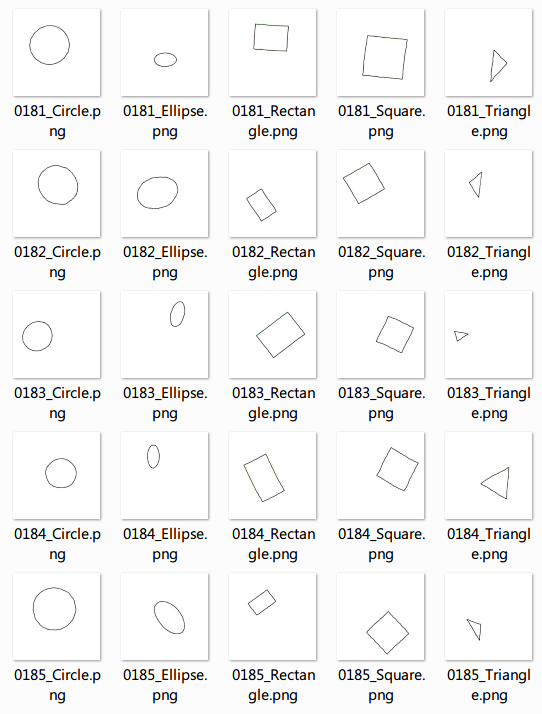
\includegraphics[width=\columnwidth]{Figure_1_CG_Image.png}
\caption{Computer-generated Images}
\end{figure}

\subsubsection{Hand-drawn Sketches}

The sketches drawn by one (under development) difference person(s) look like this (Figure 2).

\begin{figure}[ht!]
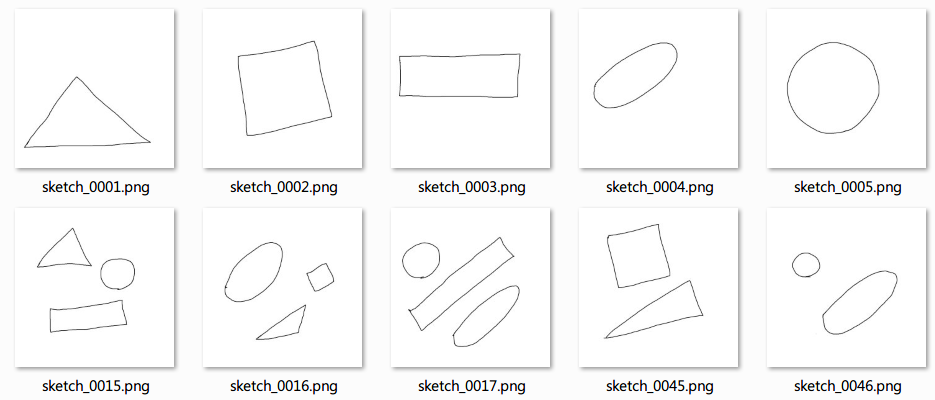
\includegraphics[width=\columnwidth]{Figure_2_Sketch_Image.png}
\caption{Hand-drawn Sketches}
\end{figure}

